\subsection{Wykresy zbiorów}
\begin{figure}[!ht]
    \centering
    \begin{subfigure}{.5\textwidth}
      \centering
      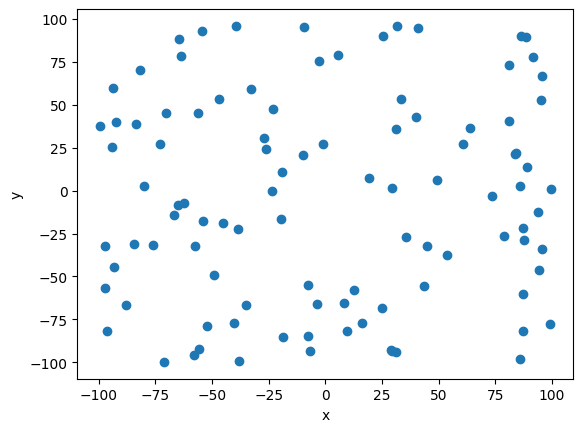
\includegraphics[width=.9\linewidth]{a.png}
      \caption*{Rys. 1: Zbiór $a$.}
      \label{fig:sub1}
    \end{subfigure}%
    \begin{subfigure}{.5\textwidth}
      \centering
      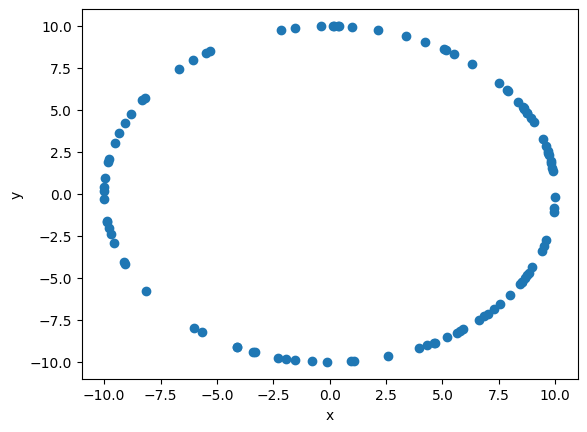
\includegraphics[width=.9\linewidth]{b.png}
      \caption*{Rys. 2: Zbiór $b$.}
      \label{fig:sub2}
    \end{subfigure}
    \label{fig:test}
    \end{figure}
    
    \begin{figure}[!ht]
    \centering
    \begin{minipage}{.5\textwidth}
      \centering
      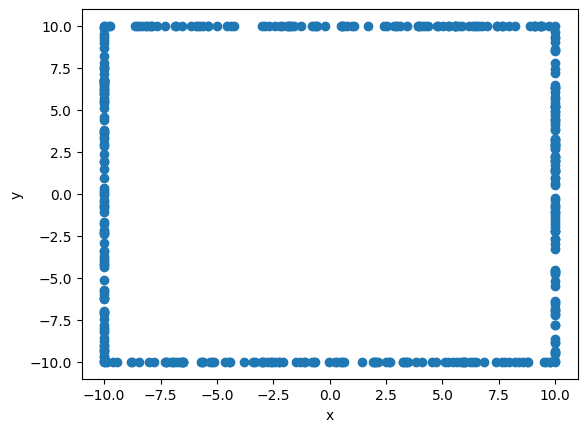
\includegraphics[width=.9\linewidth]{c.png}
      \caption*{Rys. 3: Zbiór $c$.}
      \label{fig:test1}
    \end{minipage}%
    \begin{minipage}{.5\textwidth}
      \centering
      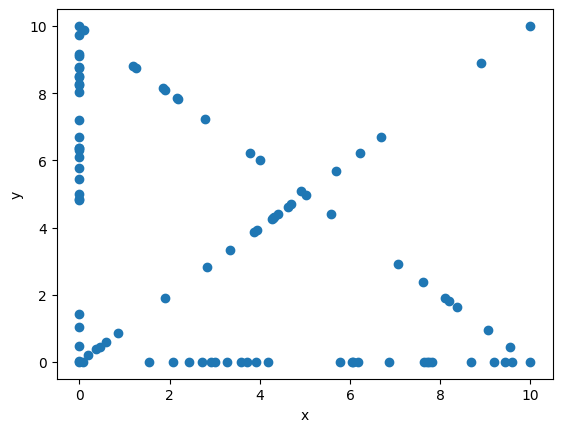
\includegraphics[width=.9\linewidth]{d.png}
      \caption*{Rys. 4: Zbiór $d$.}
      \label{fig:test2}
    \end{minipage}
    \end{figure}
\null
    \subsection{Algorytmy generacji zbiorów}
    \begin{enumerate}
    \item Dla zbioru $a$. Osobna generacja każdego z lososwych punktów.
    \item Dla zbioru $b$. Parametryzacja punktów na okręgu za pomocją funkcji trygonometrycznych $\sin$ i $\cos$.
    \item Dla zbioru $c$. Osobna generacja każdego z lososwych punktów leżących na bokach prostokąta.
    \item Dla zbioru $d$. Generacja punktów leżących na bokach kwadratu w podobny sposób do 
    zbioru $c$, dla przekątnych - generacja parametryzacja jednej ze wspólrzędnych za pomocą drugiej.
    \end{enumerate}